\chapter{Introduction}
\label{cha:introduction}

The purpose of this chapter is to provide an overview of the context, goals, and
core principles that serve as foundations for the overall cluster architecture,
both theoretical and implemented. \\ %
These so-called foundations are not restricted to this project and/or
environment, but can be considered as the minimum requirements and principles to
obtain a greener, energy and resource-aware software in general that is not only
for the present, but also, and must be, for the future, because we, as the overall
ICT community, have mostly ignored them in the past without giving them the
appropriate weight.

reCluster is heterogeneous because it is composed of numerous and diverse
components, ranging from computers to networking equipment, that have been
reutilized after decommissioning. The fundamental goal of reCluster is to establish
a cluster (hence the name) without reinventing the wheel, but rather to increase
reusability by transforming and adapting heterogeneous hardware and software
components designed for similar environments, enhancing the overall reduction of
both energy consumption and resources involved without compromising overall performance,
responsiveness, and ease of use.

\section{Context}
\label{sec:introduction_context}

Most existing systems rely entirely on large data centers, which are excessively
energy-hungry and do not provide any resource awareness owing to virtualization/abstraction
layers. Furthermore, the servers are maintained permanently powered on to significantly
minimize the time necessary for provisioning client instances while achieving virtually
100\% uptime\footnote{\url{https://aws.amazon.com/it/compute/sla}}\footnote{\url{https://azure.microsoft.com/support/legal/sla}}\footnote{\url{https://cloud.google.com/compute/sla}}.
\\ %
To achieve a greater degree of sustainability, the time necessary for provisioning
must be rebalanced, allowing servers to be completely powered off while
maintaining a similar level of uptime. It should be highlighted that this is ideal
for many applications that may be classified as non-critical, while critical
applications, such as emergency response and payment systems, require "five nines"
or 99.999\% or around five minutes and 15 seconds of downtime per year\footnote{\url{https://aws.amazon.com/blogs/publicsector/achieving-five-nines-cloud-justice-public-safety}}.

Radovanovi\'{c} et al., in \cite{carbon_aware_computing_datacenters}, describe
Google's Carbon-Intelligent Compute Management system, which actively reduces electricity-based
carbon footprint and power infrastructure costs by deferring temporally flexible
workloads. It uses a collection of analytical pipelines to acquire the next day's
carbon intensity projections, train day-ahead demand prediction models, and
apply risk-aware optimization to generate the next day's carbon-aware capacity
for all Google data centers. The system limits the resources available to temporally
flexible workloads on an hourly basis while preserving overall daily capacity,
allowing all such workloads to be completed within a day. \\ %
This type of computing solution only accounts for services and processes that
can be delayed, not those that must be continually active with an acceptable response
time; sending a critical email that is only delivered the following day is
unacceptable. It is only compatible with Google's data centers and does not provide
a more interoperable solution that is compatible with other data centers.
Moreover, the code is closed source, which means it does not adhere to the FLOSS
philosophy. Nevertheless, the notion of deferring non-real-time operations, employing
analysis and projections, to be rescheduled when the system is underutilized, improving
overall sustainability and lowering the costs, should be considered.

Enes et al., in \cite{power_budgeting_big_data_applications}, present a platform
that manages a power budget to limit the amount of energy spent by users,
applications, and individual container instances. The energy constraint is
accomplished by the platform's capability to monitor container energy
consumption and dynamically modify its CPU and memory resources via Vertical
Scaling as necessary (see section \ref{subsec:implementation_autoscaling_vertical_pod_autoscaler}).
\\ %
This approach is much more high-level and directly autoscale the resources
allocated to containers based on the power allocation among users and
applications, as opposed to a low-level approach that involves physically terminating/bootstrapping
the server (used by reCluster). Moreover, the energy is viewed as a precious resource
that can be split and shared, improving the container system's overall awareness
of its resources. Nevertheless, it needs to be combined with additional
approaches to achieve high and low levels of energy awareness and reduction.

Paya and Marinescu, in \cite{energy_aware_load_balancing}, presented an energy-aware
operation model for load balancing and application scaling on a cloud, outlining
an energy-optimal operation regime and aiming to increase the number of servers employed
in this regime. Servers that are idle or only barely loaded are put into one of
the sleep modes to conserve energy. Therefore, the following could be employed
to reformulate the conventional idea of load balancing in a large-scale system: \textit{"Distribute
evenly the workload to the smallest set of servers operating at optimal or near-optimal
energy levels, while observing the Service Level Agreement (SLA) between the Cloud
Service Provider (CSP) and a cloud user. An optimal energy level is one when the
performance per Watt of power is maximized"}. \\ %
To reduce energy waste, this approach can be applied to an external load balancer
employed in the architecture. Even more, energy can be saved by completely turning
off mostly inactive or lightly-loaded servers rather than switching them into sleep
mode. This new type of load balancer can also be interfaced with the Cluster
Autoscaler and Server to better understand the overall cluster state, both in terms
of active/inactive nodes and also of overall power consumption, to obtain more
fine-grained information and therefore increase the overall efficiency.

All of the above strategies attempt to minimize energy consumption in various
contexts: non-real-time services, containerization, and load balancing. Yet, none
of them address, or only partially address, the core cause of the highest energy
usage in a cluster architecture, which is the server themselves. To establish a more
sustainable and resource-aware cluster, the servers must be considered and
therefore autoscaled by physically bootstrapping or terminating them; since a powered-off
machine consumes (nearly) zero energy. \\ %
Nonetheless, the prior techniques should, and must, be extended into future
versions of reCluster to achieve even higher levels of energy reduction while
satisfying the SLA. \\ %
More than ever, a more sustainable cluster architecture is required.

\section{Goals}
\label{sec:introduction_goals}

A cluster is composed of several components, including hardware and software,
that operate together as a single entity to accomplish one homogeneous goal, or multiple
and different goals. The hardware components, which are typically computers of different
kinds ranging from desktop computers to single board computers, are connected in
a single network: the cluster network, by additional hardware components
particularly designed for communication. Because multiple applications can achieve
the same result, are constantly evolving with newer features and capabilities, and
can be employed or not depending on the (current) needs and requirements, the
software components can vary and are as heterogeneous as the hardware, if not more.
Between hardware and software, two major distinctions complement one another.
The first distinction is that hardware, particularly reconditioned hardware, is
limited in its ability to be modified and transformed, whereas software is essentially
limitless in this regard and may achieve the same goal using multiple technologies
and/or languages. The second distinction is that there is no difference between
the various hardware components in terms of whether they are used for cluster
operations or user operations. Instead, software components can be divided into
low-level ones that are used to keep the overall cluster operational and high-level
ones that are used by the users for their specific services. In this context,
software in all of its aspects must be used to compensate for the shortcomings
of the hardware since it can be customized to fill the gaps where the hardware
lacks. \\ %
Most used hardware components may be reconditioned by reusing decommissioned
components from consumers and organizations due to upgrades. Because newer components
are often more performant and energy-efficient than older ones, the hardware is
directly and automatically managed by the various cluster-related software
deployed. \\ %
The cluster must be as simple as possible, with human interaction minimized to nearly
zero, and automatic solutions preferred. The most essential automated solution that
must be implemented in a cluster is autoscaling, both upscaling and downscaling.
In upscaling, the cluster automatically bootstraps an inactive hardware
component. Whereas in downscaling, the cluster automatically terminates an
active hardware component. Selecting which component(s) to autoscale can follow
multiple criteria, such as choosing nodes that are more power efficient or performant,
or even a combination of the two. The latter is an excellent illustration of the
combination of hardware and software that needs to be present in the cluster. \\ %
The cluster should be used in a wide range of environments and use-case scenarios,
from a modest and local deployment at home to a large and remote deployment
comparable to that found in a data center. Given that the various software manages
them automatically using the autoscaling technique, there should be no limit to
the number of involved computers. \\ %
If there is no need to operate the cluster for specific periods and it is
therefore considered worthless, it can be completely shut down, with the benefit
of reducing its overall power consumption to zero. When it is necessary again,
it is reactivated. Although the latter may create some performance and/or responsiveness
issues, because no physical machines are managing any service, it is far preferable
to an always-on technique. The latter impacts can be mitigated if the
organization can calculate different models and/or employs a single board
computer as the always-on hardware component thanks to its overall extremely low
power consumption. As stated previously, the context is dynamic, and hence the latter
is dependent on the organization in charge of the cluster.

As a result, the cluster should appear less heterogeneous and more like a
homogenous, and mostly automated entity.

\section{Principles}
\label{sec:introduction_principles}

This section is dedicated to illustrating some of the fundamental principles
around which the overall design is based. These principles should be seen as the
foundations for a more sustainable, resource-aware, free and open-source, and
energy-efficient architecture that may be utilized not only in this specific
context, but in all aspects of ICT. \\ %
It should be highlighted that these principles should not be regarded as negative
to overall performance and responsiveness, but rather as equally important. Performance
and responsiveness currently constitute the sole and most significant characteristics
to consider when examining software, but in the future, it should be necessary,
almost mandatory, to include, maybe gradually but starting to consider them as
parameters for comparisons and essential aspects of a program. \\ %
The applicability of these principles is determined by the organization's
requirements. Yet, some of these principles should be investigated and
implemented in the future for greener and more resource-aware software. \\ %
The proposed list can undoubtedly be improved upon and/or expanded with
additional, and possibly more strict, principles. Shifting the computing industry
toward a more sustainable future should be possible, if not essential.

\subsection{Sustainability}
\label{subsec:introduction_principles_sustainability}

\begin{wrapfigure}
  {l}{.2\textwidth} %
  \centering
  \def\stackalignment{l}\stackunder{ 
\includegraphics[width=\linewidth]{images/logos/sdgs.png} } %
  {\scriptsize \parbox[t]{\linewidth}{ Source: \url{https://www.un.org/sustainabledevelopment/news/communications-material}} }
\end{wrapfigure}

The United Nations (UN) has established 17 Sustainable Development Goals\footnote{\url{https://sdgs.un.org}}
(SDGs). The SDGs address climate change and strive to preserve the oceans and forests,
while also addressing poverty and other deprivations via initiatives that
improve health and education, reduce inequality, and stimulate economic growth. \\ %
Clearly, in an ICT context, several of these Goals may appear to be out-of-context,
unreachable/unfeasible, or not directly related. However, the majority of them, including
those that are not directly related to an ICT context, must be considered when
developing new software applications and architectures; given that a minor improvement
in a single SDG can benefit all other SDGs. There is no need to change or
entirely disrupt a project's primary goal, but rather to integrate the relevance
of these long-term goals into the development process. If an ICT initiative
improves or enhances one or more SDGs, it will undoubtedly benefit not only other
direct and associated SDGs, but practically every other SDG as well. \\ %
A large end goal is nearly always comprised of a plethora of many smaller
improvements/objectives that, when considered separately, may appear to be
irrelevant, but when placed together form a sustainable chain of progress.

\subsection{Acknowledging Planetary Limits}
\label{subsec:introduction_principles_acknowledging_planetary_limits}

\begin{wrapfigure}
  {l}{.2\textwidth} %
  \centering
  \def\stackalignment{l}\stackunder{ 
\includegraphics[width=\linewidth]{images/introduction/limits.png} } %
  {\scriptsize \parbox[t]{\linewidth}{ Icon made by \href{https://www.flaticon.com/authors/freepik}{Freepik} from \href{http://www.flaticon.com}{www.flaticon.com} }}
\end{wrapfigure}

When available resources are limited, it is essential to preserve them and
reduce their overall consumption as much as possible. It is important to note that
the term resources in this context is more generalized and does not designate any
specific resource type, but they may be regarded as a distinct entity that
groups them. \\ %
Rethink and change the availability of resources, and investigate a more realistic
and conservative approach, referred to in \cite{computing_within_limits} as
computing within limits or simply LIMITS. LIMITS incorporates three major topics:
present and near-future ecological, material, and energy constraints; new forms of
computing that may assist promote well-being while living within these limits;
and the influence of these limits on the area of computing. Not only is the concept
of LIMITS confined within a computing environment, but it also aims to integrate
other, and sometimes uncorrelated, heterogeneous areas. Moreover, because
resources are not exclusively available to individuals, there is a need to think
about and focus on collectives and larger contexts engaging in stronger connections
to sustainable activities in disciplines other than computing. The term resource(s)
should be considered not just to describe actual elements, but also to encompass
socioeconomic, more intangible, factors that may be enhanced by diverse
techniques pursued by the computing community, such as promoting development rather
than economic growth. \\ %
As stated in \cite{ed_tech}, the incorrect underlying assumptions of endless, infinite,
and replicable technological resources must be reconsidered. These assumptions are
just unsuitable for a more constrained and sustainable future. To re-imagine how
digital technologies may be developed and implemented in these new and limited
computing architectures, new concepts of radically leaner and ecologically conscious
techniques are necessary. \\ %
Another element of the architecture's involved resources is the relationship between
the software and the hardware. Because of the current amount of processing power,
some software has ridiculously high hardware requirements for even the most simple
operations. Better and more performant programming languages and algorithms need
to be employed to rethink, modify, and/or improve software resource requirements.
A different technique is necessary with the adoption of a more permacultural approach,
which is referred to as permacomputing in a computing environment. Permacomputing,
as depicted in \cite{permacomputing}, is both a concept and a community of practice
centered on issues of resilience and regenerative in digital technology,
transforming problems into solutions, competition into cooperation, and waste
into resources. \\ %
Transform what appears to be a disadvantage, a difficulty, or even a waste into
a rich and valuable resource.

\subsection{Hardware Reusability}
\label{subsec:introduction_principles_hardware_reusability}

\begin{wrapfigure}
  {l}{.2\textwidth} %
  \centering
  \def\stackalignment{l}\stackunder{ 
\includegraphics[width=\linewidth]{images/introduction/recycle.png} } %
  {\scriptsize \parbox[t]{\linewidth}{ Icon made by \href{https://www.flaticon.com/authors/freepik}{Freepik} from \href{http://www.flaticon.com}{www.flaticon.com} }}
\end{wrapfigure}

Use reusability and repairability approaches to reduce resource waste as much as
possible. \\ %
The majority of unused hardware is perfectly capable of fulfilling the majority
of tasks and operations in sustainable architecture, such as hosting a website or
a cache server, without any particular difficulty. Unused hardware is frequently
created by an upgrade to a newer and more recent version or by (major) scheduled
decommissioning. \\ %
Typical electronic devices with even a single faulty hardware component are discarded
and promptly replaced with newer hardware, even if the remaining components are
healthy and completely functional. The expenses and work required for a repair vary
depending on the device, but most of the time the repair may be performed
quickly and cheaply by replacing the faulty component with a new one. Furthermore,
and this is especially true for desktop computers, if two devices are compatible
and one has some broken components that the other does not, the healthy
components can be combined to re-create a single but healthy and usable device
with the benefit of drastically reducing the overall amount of resource waste. \\ %
The latter two approaches not only recycle abandoned technology but also reduce
the overall quantity of electronic waste (e-waste) that they can generate. Consequently,
the energy gap between overall utilization energy and production energy, formerly
expressed as embodied energy, can be narrowed or even attained and exceeded. \\ %
Yet, the ease and feasibility of a device's repairability is entirely dependent on
its manufacturer. Moreover, there are cases where the devices have a planned obsolescence
after which some of the components will probably break and the cost or effort required
for a repair is unfeasible, and it is far easier to buy a new one while
discarding the old and broken one, causing additional (e-)waste. It is difficult
to avoid the latter, and almost certainly additional issues, induced by the
manufacturer. Yet, in recent years, there have been an increasing number of consumer
activities aimed at reducing or eliminating the behaviors perpetuated by these manufacturers.
The Right To Repair\footnote{\url{https://www.repair.org}}\footnote{\url{https://repair.eu}}
movement is the most well-known, to advocate for repair-friendly policies,
regulations, statutes, and standards. Another approach is to provide a repairability
index, such as the French repair index\footnote{\url{https://www.ecologie.gouv.fr/indice-reparabilite}},
for the products so that potential customers may know and understand how easy it
is to repair the corresponding device before purchase. It should be noted that
not all manufacturers are opposed to repairability, and there are certain,
albeit small, manufacturers, such as Framework\footnote{\url{https://frame.work}},
that have repairability as one of their core missions, building longevity
products and improving the overall availability of spare parts and ease of
upgrade, customization, and repairability. The objective/hope is that more manufacturers
will begin to design, produce, and distribute more sustainable products. \\ %
Instead of planned obsolescence, consider planned longevity.

\subsection{Energy Reduction}
\label{subsec:introduction_principles_energy_reduction}

\begin{wrapfigure}
  {l}{.2\textwidth} %
  \centering
  \def\stackalignment{l}\stackunder{ 
\includegraphics[width=\linewidth]{images/introduction/energy.png} } %
  {\scriptsize \parbox[t]{\linewidth}{ Icon made by \href{https://www.flaticon.com/authors/freepik}{Freepik} from \href{http://www.flaticon.com}{www.flaticon.com} }}
\end{wrapfigure}

The architectures and software should strive to reduce their total energy
footprint as much as possible while providing similar, if not identical,
outcomes. Concerning the preceding point, this is only possible if the
organization has complete control over all aspects of the architecture, since the
union of software and hardware is the only conceivable and feasible strategy to establishing
a more sustainable and energy-aware architecture. \\ %
Energy is one of the most significant factors in achieving sustainable architecture.
Because energy is closely related to carbon emissions, there is a need for low-carbon
and sustainable computing with a path towards zero-carbon computing, as stated
in \cite{frugal_computing}, because current computing emissions account for about
2\% of global emissions and are expected to rise dramatically in the upcoming
years. This rate of expansion is unsustainable and as a community, we must begin
to regard computational resources as finite and valuable, to be used only as essential
and as effectively as possible. The latter is known as frugal computing, and it strives
to get the same outcomes while using less energy by being more frugal with the available
computing resources. In the current context, for example, if a system/computer
in a cluster is not needed or is underutilized, it is a waste of both energy and
resources. It must be terminated and, if any services are deployed on it,
migrated to another active system to avoid service interruptions, increasing its
utilization and lowering the architecture's total power consumption while maintaining
the same level of Quality of Service (QoS). Humans are unable to perform these
operations since there is the need to continuously monitor and check the overall
status of the entire architecture. The core principles of energy reduction must be
developed into automatic systems that could be easily extended to existing applications
and tools which are focused solely on overall system performance and responsiveness.
The system should be as efficient as possible, employing only those components that
are strictly necessary, avoiding bootstrapping unneeded machines and terminating
those that are unnecessary, and avoiding the paradigm of an always-on architecture
that wastes energy and resources. \\ %
Another factor to consider is the embodied energy of each hardware system.
Embodied energy is the energy necessary to build all of the electronic
components (both network and especially consumer appliances). It emerges that the
energy used to manufacture electronic components is significantly higher, and in
many cases dominant, than the energy needed throughout their whole operation\cite{monster_footprint}.
This means that practically every hardware component is underutilized in terms of
the energy required for manufacturing it. As a result, there is a need to correct
this imbalance by attempting to reach at least the same amount of energy. It
should be noted that the latter does not want to employ the hardware
unconsciously, but rather with better and more conscious principles and logic that
not only tries to reduce the overall "live" energy consumption, but also tries
to equal, if not even surpass, the embodied energy of each electronic device
that is employed in the architecture. \\ %
Previously, the term carbon emission/footprint was used concerning energy consumption.
Yet, it is necessary to accurately define how the overall energy of the architecture
is estimated, as well as the fundamental principles on which the calculation is
based. This is not as simple as it appears. \cite{world_wide_web_carbon} reveal
that quantifying the carbon footprint has produced contradictory results, implying
the need for different and alternative approaches that delineate the specific relationships
between elements - geographic, technical, and social - within the broader information
and communication technologies infrastructure. The common method of assessing
the energy impacts is the kilowatt hours of electricity and gigabytes of data
through a network, expressed as the functional unit \texttt{KWh/GB}. The \texttt{KWh/subscriber}
metric, which divides the larger energy draw inside a study's system boundary by
the number of subscribers within the network, can better represent worldwide
patterns in network access expansion over time. Rather than calculating \texttt{KWh/GB}
or \texttt{KWh/subscriber}, a relational approach would assess the carbon, water,
and land footprints of powering the whole architecture in specific regions of
the world, highlighting the significant disparities between the various locations.
Network shapes, rather than scales, provide new possibilities for assessing the
existing and future Internet\cite{world_wide_web_carbon}.

\subsection{Insourcing}
\label{subsec:introduction_principles_insourcing}

\begin{wrapfigure}
  {l}{.2\textwidth} %
  \centering
  \def\stackalignment{l}\stackunder{ 
\includegraphics[width=\linewidth]{images/introduction/insourcing.png} } %
  {\scriptsize \parbox[t]{\linewidth}{ Icon made by \href{https://www.flaticon.com/authors/kerismaker}{kerismaker} from \href{http://www.flaticon.com}{www.flaticon.com} }}
\end{wrapfigure}

Invert the trend of constantly outsourcing applications to third-party cloud providers;
we might express this with a neologism: "Insourcing". \\ %
While there are undeniable benefits to outsourcing in terms of convenience and better
pricing, it erodes institutional and human independence by centralizing a single
point of failure and delegating relevant choices regarding privacy, data ownership,
and environmental impact on these external actors\cite{conceptualising_resource_aware}.
\\ %
There is a need to obtain, direct control over the whole software stack, beginning
with the hardware infrastructure and progressing through the application's development
and final release. At first look, reversing the ICT outsourcing trend may appear
to be impracticable, unneeded, and comparable to an old and mostly outdated approach.
Nonetheless, overall technology, tools, and usability have significantly improved
in recent years. Most importantly, there has been a shift in the software community
toward standardization and interoperability across heterogeneous systems, which
has not only made deploying software locally and with an in-house infrastructure
trivial, but has also aided in abstracting away from the final user common and not-so-trivial
problems, such as handling and coordinating multiple connections across
different hardware and software components/layers. \\ %
As discussed in \cite{precarious_infrastructure} current infrastructures and
approaches to climate change are mitigation-oriented, aiming only to support or investigate
social changes that reduce the material causes of the more pernicious facets of global
change, with the implicit assumption that these infrastructures will persist as
the risks of current unsustainable practices become urgent threats to well-being
and survival. Instead, new architectures, and possibly old ones through refactoring
and rethinking the overall design, must take and address new approaches, denoted
as post-apocalyptic computing, to address the many, dramatic, and complex
phenomena associated with global change, allowing to prepare for nonlinear changes.
If the organization has direct control over almost every aspect of the
architecture, the latter can be accomplished with almost negligible effort,
whereas if everything is outsourced to an external entity, the organization has only
a limited amount of control over the possible future outcomes that can arise from
unpredictable changes that will occur sooner or later. As a result, avoid remote
and generally unknown architectures of third-party organizations that only raise
the fragile state on which the application is deployed, establishing an inherent
single point of failure that not only can be an issue for the present but, more significantly,
for the future. \\ %
Another significant aspect of current architectures and approaches is that most
operations are performed remotely and outsourced to external organizations, even
though the participating entities are mostly close together, resulting in extra
workload and networking equipment, which translates to an increased amount of overall
power consumption. In this regard, the usage of external videoconferencing applications
that enable remote entities to connect is a significant example. When two close
entities, that can be even in the same building, seek to establish a
teleconference, their data is routed to remote videoconferencing servers.
Instead of depending on an external and remote service, it is possible to set up
a local videoconferencing service in the local (insourced) architecture,
employing open-source software and improving overall security and privacy. The distance
between the entities and the local server instance may be drastically reduced,
decreasing latency and lowering total power consumption for the videoconference,
as theorized in \cite{comparison_energy_carbon_time_videoconferencing},
resulting in better outcomes and more sustainable service. \\ %
Lastly, insourcing enables better fine-grained and conscious control over the whole
application's data and everything that comes with it, such as privacy and
security, because it is known where and how it is stored, distributed, and protected.
Even though these later elements are not the primary focus of this document, they
should not be ignored or underestimated because they are essential for almost every
software application. Furthermore, various initiatives in recent years have attempted
to improve data protection for individuals and organizations, including the well-known
General Data Protection Regulation\footnote{\url{https://gdpr.eu}} (GDPR)
drafted and passed by the European Union (EU). \\ %
As a result, returning to an insourcing approach and having direct control over almost
every aspect of the architecture and software stack is not only feasible and almost
trivial nowadays, but also necessary for establishing a better and more
sustainable future for everybody, not just the individual.

\subsection{Interoperability}
\label{subsec:introduction_principles_interoperability}

\begin{wrapfigure}
  {l}{.2\textwidth} %
  \centering
  \def\stackalignment{l}\stackunder{ 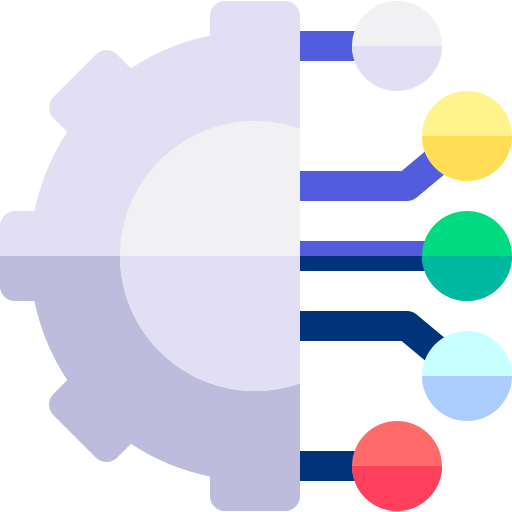
\includegraphics[width=\linewidth]{images/introduction/interoperability.png} } %
  {\scriptsize \parbox[t]{\linewidth}{ Icon made by \href{https://www.flaticon.com/authors/freepik}{Freepik} from \href{http://www.flaticon.com}{www.flaticon.com} }}
\end{wrapfigure}

Interoperability and standardization of hardware and software must be at the core
of a more sustainable architecture. Most, if not all, of the components, employed
in the design must agree on common interfaces to prevent the need for hardware adapters
and software translation layers, which not only increase resource waste and
energy consumption but also decrease overall system performance. \\ %
When all of the applications employed by the architecture agree on or adapt to a
common set of interfaces, achieving software interoperability is virtually straightforward.
Upgrading previously incompatible software is feasible, albeit depending on the complexity
of the program, refactoring may be required. Fortunately, most software programs
and, more broadly, the computing environment depends on standards that are
equivalent in practically every part of the world. Consider the Internet itself,
which is built on standards and interoperability between all sorts of
heterogeneous components. \\ %
On the other hand, implementing hardware interoperability and standardization is
considerably more challenging than software since it is heavily dependent on design
decisions made by the manufacturer throughout the development phases. As a
result, there is a need to persuade, mostly through legislation, the many manufacturers
that are reluctant to adapt and do not meet or do not want to establish a set of
standards that improve interoperability on their devices. A perfect example of
the latter is the European Parliament's approval of a law, following an impact assessment
study\footnote{\url{https://data.europa.eu/doi/10.2873/528465}}, that mandates
by the end of 2024 a common, standardized, and interoperable charger for all
mobile devices sold in the EU internal market\footnote{\url{https://www.europarl.europa.eu/news/en/press-room/20220930IPR41928/long-awaited-common-charger-for-mobile-devices-will-be-a-reality-in-2024}}.
The latter has been highly awaited, and it may be regarded as a first step
toward a much broader trend of standardization and interoperability that can
establish the foundation for a more sustainable future. \\ %
Furthermore, they can significantly reduce the effort required while also increasing
the ease of establishing an insourcing architecture. Various organizations can
exploit a uniform and de-facto standard that enables high-level interoperability
between heterogeneous architectures, accelerating the process of migrating various
services and deployments from remote to local architectures. \\ %
Lastly, having an interoperable architecture, combining software and hardware,
eliminates the so-called technology vendor lock-in effect, in which a customer is
dependent on a single manufacturer. Because the entire architecture might be
composed of reconditioned/refurbished hardware and thus is intrinsically
heterogeneous, the vendor lock-in effect cannot be tolerated.

\subsection{Free/Libre And Open Source Software}
\label{subsec:introduction_principles_free_libre_and_open_source_software}

\begin{wrapfigure}
  {l}{.2\textwidth} %
  \centering
  \def\stackalignment{l}\stackunder{ 
\includegraphics[width=\linewidth]{images/logos/open_source.png} } %
  {\scriptsize \parbox[t]{\linewidth}{ Source: \url{https://opensource.org/logo-usage-guidelines}} }
\end{wrapfigure}

The software developed and employed in the architecture must be Free/Libre and Open
Source in all aspects. If a software application is incompatible with the latter,
an alternative must be identified or developed. \\ %
Following the GNU Project's philosophy\footnote{\url{https://www.gnu.org/philosophy}}:
\textit{Free Software means that users have the four essential freedoms: (0) to run
the program, (1) to study and change the program in source code form, (2) to redistribute
exact copies, and (3) to distribute modified versions.} \\ %
This principle's fundamental is presented as Free/Libre and Open Source Software\footnote{\url{https://www.gnu.org/philosophy/floss-and-foss.html}}
(FLOSS). \\ %
Being FLOSS-compatible has also the significant advantage of allowing external programmers
to contribute to the software, consequently improving overall quality and
providing for more performant and efficient logic and algorithms.

\subsection{Dependencies Reduction}
\label{subsec:introduction_principles_dependencies_reduction}

\begin{wrapfigure}
  {l}{.2\textwidth} %
  \centering
  \def\stackalignment{l}\stackunder{ 
\includegraphics[width=\linewidth]{images/introduction/packages.png} } %
  {\scriptsize \parbox[t]{\linewidth}{ Icon made by \href{https://www.flaticon.com/authors/freepik}{Freepik} from \href{http://www.flaticon.com}{www.flaticon.com} }}
\end{wrapfigure}

For decades, as stated in \cite{software_dependency_problem}, discussion about
software reuse was more widespread than real software reuse. Nowadays, the
situation is reversed, with developers reusing software produced by others regularly
in the form of software dependencies, and the situation is largely unexamined. Software
dependencies pose substantial risks that are all too often ignored. The
transition to easy, fine-grained software reuse has occurred so quickly that there
is little knowledge of the best practices for identifying and using dependencies
effectively, or even determining when they are appropriate and when they are not.
Installing a package as a dependency outsources the effort of developing that code
--- designing, writing, testing, debugging, and maintaining --- to someone else on
the Internet that is mostly unknown. Using that code exposes the program to all
of the problems and weaknesses in the dependency. Therefore, if a dependency
appears to be too problematic and there is no easy or effective procedure to
isolate it, the best solution may be to avoid it totally, or at least the parts
that have been recognized as the most dangerous. \\ %
The latter is essential to acquiring a critical perspective on the dependencies
used in the overall architecture. There is a need to evaluate the real and unreplaceable
dependencies and avoid those that are unnecessary and too critical to be adopted
by the architecture. Thinking about future design with a more LIMITS, post-apocalyptic,
and mostly resource-aware perspective should begin from the foundation. Lowering
and simplifying the software stack's core and external dependencies significantly
minimizes the time required to maintain and deploy it.